\section{Carica}
\subsection{Carica Elettrica}
    Per le cariche elettriche sono presenti due modelli matematici per descrivere la loro distribuzione dello spazio:
    \begin{itemize}
        \item Cariche puntiformi: modello discreto
        \item Distribuzione di carica: modello continuo
    \end{itemize}

    È importante definire una variabile fisica chiamata carica contenuta: è la carica contenuta in un volume v ($q^c[t,v]$ con $q^c$ funzione del volume v e si esprime in Coulomb).\\
    $q^c$ è una variabile globale, cioè dipende dalla scelta di un elemento geometrico v che descrive il volume.\\
    Si può quindi definire la densità volumica di carica $\rho_c$. Per definire questo elemento si ipotizza che la \textbf{carica si distribuisca uniformemente in v}. \\
    \begin{center}
        $\rho_c(t,p) := \frac{q^c[t,v]}{v}, \rho \in v [\frac{C}{m^3} ]$\\
    \end{center}
    Come è logico pensare, la carica solitamente \textbf{NON} si distribuisce uniformemente.

    \subsubsection{Principio di uniformità}
        INSERIRE GRAFICO\\
        Se si considera un intervallo infinitesimo in un intorno del punto P, anche la variazione della funzione in quell'intorno sarà infinitesima. Per grandezze infinitesime, quindi, si può assumere che le grandezze siano uniformi e costanti.

        Applicando il \textbf{principio di uniformità} alla determinazione di $\rho_c$ ne caso generale:
        \begin{enumerate}
            \item prendiamo un punto $P \in v$
            \item prendiamo un \textbf{cubo centrato in P}
            \item $\lim_{v' \to 0} \rightarrow 0$
            \item nel $v'$ la carica si distribuisce uniformemente
            \item applichiamo la definizione di $\rho_c$ nel caso di distribuzione uniforme a $v'$\\
            \begin{equation}
                \rho_c[t,P] := \lim_{v' \to 0} \frac{q^c[t,v']}{v'} = \frac{dq(t,p)}{dv}
            \end{equation}
            \item effettuare la stessa procedura per qualsiasi punto dentro v
        \end{enumerate}

Si ottiene così un \textbf{campo scalare} $\rho_c(t,\mathbf{P})$: per ogni punto $\mathbf{P} \in V$, $\rho_c$ restituisce uno scalare (densità volumetrica). All'interno di un volume:
\[
q^c[t,\tau] = \int_\tau \rho_c(t,\mathbf{P}) \, dv
\]

La densità superficiale di carica è definibile come:
\[
\sigma_c(t,\mathbf{P}) := \frac{dq(t,\mathbf{P})}{ds}
\]
\[
q^c[t,\Sigma] = \int_\Sigma \sigma_c(t,\mathbf{P}) \, ds
\]
con $\Sigma$ superficie. Ovviamente è anche ricavabile l'espressione per la densità lineare di carica:
\[
\lambda_c(t,\mathbf{P}) := \frac{dq(t,\mathbf{P})}{dl}
\]
dove $dl$ è un elemento di linea infinitesimo centrato in $\mathbf{P}$.

\subsection{Classificazione delle cariche}
\begin{enumerate}
    \item \textbf{Carica libera}: carica che si muove in un corpo $q_l$ [C] (il corpo può essere un conduttore: materiale che possiede carica libera).
    
    \item \textbf{Carica legata}: può solo ruotare, non muoversi. $q_P$ [C]. È visibile negli \textbf{isolanti}, cioè i materiali che non hanno carica libera in quantità apprezzabile. Gli isolanti che presentano carica legata si dicono \textbf{dielettrici} (molecole polari).
    
    \item \textbf{Carica totale}: $q = q_t = q_l + q_P$ [C]
\end{enumerate}

\section{Come descrivere matematicamente le cariche}
Introducendo una nuova variabile fisica globale detta \textbf{carica fluente} $q^f[T,S]$: è la carica che passa attraverso la superficie $S$ durante l'intervallo $T$.
\[
q^f[T,S] := \sum_i k_i q_i
\]

Per definire $k_i$ si deve orientare la superficie $S$: cioè scegliere una delle due normali ad $S$ che sono opposte ($\hat{n}$, $\hat{n}'$). Fatto ciò si può definire $k_i$:
\begin{enumerate}
    \item $k_i = +1$ se $q_i$ attraversa $S$ concorde a $\hat{n}$
    \item $k_i = -1$ se $q_i$ attraversa $S$ discorde a $\hat{n}$
    \item $k_i = 0$ se $q_i$ attraversa $S$ due volte
\end{enumerate}

$q^f$ è una variabile utile in quanto si può definire la corrente elettrica: è una variabile globale
\[
i[t,S] := \lim_{T \to 0} \frac{q^f[T,S]}{T} = \frac{dq^f[dt,S]}{dt}
\]

$i$ si misura in Ampere, è uno scalare, un numero reale. Esso può essere positivo o negativo e non ha un verso. La direzione della corrente viene presa in base all'orientamento di $S$. In questo caso $\hat{n}$ si chiama \textbf{orientamento di corrente}. La superficie in cui si vuole calcolare la corrente è arbitraria; risulta ovviamente scontato prendere una superficie che può essere comoda o significativa come ad esempio la sezione di un filo.

\subsection{Classificazione della corrente elettrica}
\begin{enumerate}
    \item \textbf{Conduzione}: moto di carica libera nei conduttori
    \item \textbf{Convezione}: la carica viene trascinata
    \item Carica che si muove nel vuoto
\end{enumerate}

Per sviluppare il modello ci poniamo nel caso più semplice con le seguenti ipotesi:
\begin{itemize}
    \item \textbf{$S$ è piana}: cioè una superficie che ha la stessa $\hat{n}$ in ogni suo punto
    \item $\mathbf{v}$, $\rho_c$ \textbf{uniformi} nello spazio, cioè hanno lo stesso valore in tutti i punti e costanti nel \textbf{tempo} (dove la prima indica la velocità delle cariche e la seconda la densità volumetrica di carica)
\end{itemize}

Considerata una copia di $S$ che chiamiamo $S'$ traslata di $\mathbf{d} := \mathbf{v}T$ (NB: $\mathbf{d} \cdot \hat{n} \neq 1$ non sono paralleli), la superficie $S$ ed $S'$ definiscono un esaedro $V$ di volume: 
\[
V = S h = S (\mathbf{d} \cdot \hat{n})
\]
Dobbiamo trovare un'espressione per $q^f[T,S]$ in funzione di $\rho_c$.\\

Tesi: la $q^f[T,S]$ è la carica fluente contenuta nel volume V
\begin{center}
    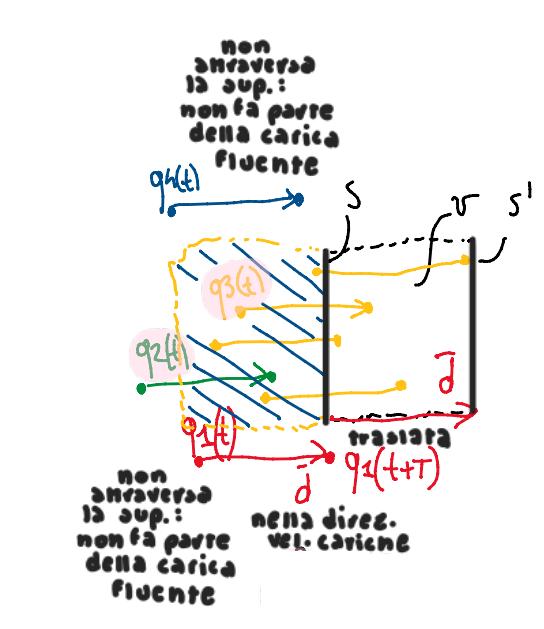
\includegraphics[scale=0.5]{immagini/image2.png}
\end{center}
\[
    q^f[T,S] = \int_v \rho_cdv = \rho_c \int_v dv = \rho_cv = \rho_cS(\overline{d}\cdot\hat{n}) = \rho_c \overline{v}\cdot\hat{n}ST
\]
\[
i[t,s] = \lim_{T \to 0} \frac{\rho_c \overline{v}\cdot\hat{n}S\not{T}}{\not{T}} = \rho_c\overline{v}\cdot\hat{n}S
\]
Si denota con $\overline{J} = \rho_c\overline{v}$ la densità di corrente e si misura in $[\frac{A}{m^2}]$. Descrive localmente il moto delle cariche.


Per ottenere un modello più generale si devono rimuovere le ipotesi semplificative che sono state fatte.\\
\begin{enumerate}
    \item Superfici curve: ogni superficie infinitesima è piana
    \item $\mathbf{v}$, $\rho_c$ costanti. Per il \textbf{principio di uniformità}: posso ritenere $\mathbf{v}$, $\rho_c$ uniformi e costanti a patto di considerare $S\to0$ e $T\to0$
\end{enumerate}

Applicando il principio di uniformità l'espressione di prima è ancora valida se consideriamo gli infinitesimi:
\[
di[t,ds] = \overline{J}(t,P)\cdot\hat{n}ds
\]
con $ds$ superficie infinitesima centrata in $P$. Se si volesse considerare una superficie $\Sigma$ non infinitesima?
\[
    i[t,\Sigma] = \int_\Sigma\overline{J}(t,P)\cdot\hat{n}(P)ds
\]
\begin{center}
    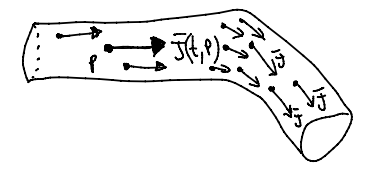
\includegraphics[scale = 0.6]{immagini/image3.png}
\end{center}

$\overline{J}$ è un campo vettoriale: torna un vettore in ogni punto $P$ del dominio.

\subsection{Come visualizzare i campi vettoriali}
\begin{center}
    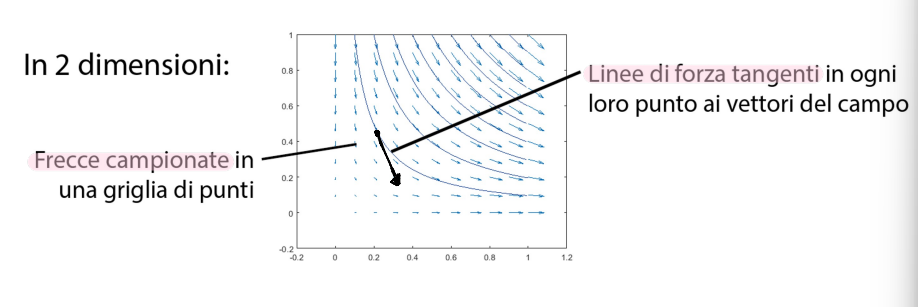
\includegraphics[scale = 0.6]{immagini/image4.png}
\end{center}
Due linee di forza ovviamente non possono sovrapporsi in quanto in un punto $Q$ è presente solo un vettore.
\subsubsection{Conduttore filiforme}
    \begin{center}
        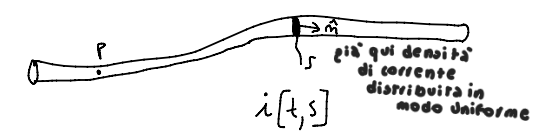
\includegraphics[width=0.5\linewidth]{immagini/image6.png}    
    \end{center}
    d è il diametro della sezione e l la lunghezza, si considera l>>d.\\
    In queste condizioni la sezione S è talmente piccola da ritenersi quasi infinitesima ed è possibile applicare il \textbf{principio di uniformità}
    \begin{center}
        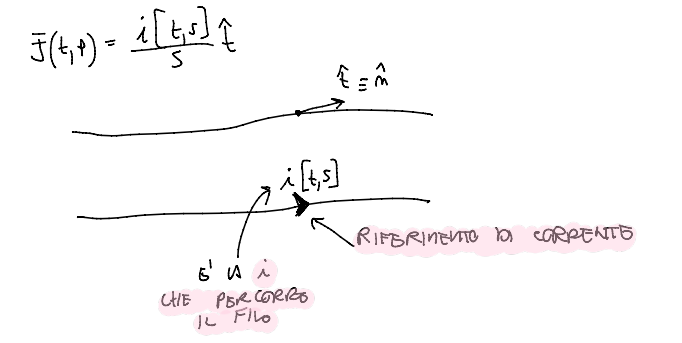
\includegraphics[width=0.5\linewidth]{immagini/image5.png}  
    \end{center}

\subsection{Legge di continuità della carica elettrica}
    Il principio di conservazione della carica: la carica non si crea e non si distrugge in quantità macroscopica.

    Il \textbf{bordo} del volume $v$ è una superficie $S=\partial v$. $\partial v$ sono superfici \textbf{chiuse}, cioè $\partial S = \partial\partial v = 0$.

    L'obiettivo è mettere in relazione la carica contenuta in $v$ con la carica fluente dal suo bordo. La variazione di carica contenuta corrisponde alla carica fluita all'esterno del volume.
    \[
        q^f[t,\partial v] = q^c[t,v] - q^c[t+T,v]
    \]
    Cariche fluite attraverso il volume = differenza di carica tra l'inizio (t) e la fine dell'intervallo (t+T)
    \[
        q^f[T,\partial v] = \int_T i[t,\partial v]dt = i[t, \partial v]\cdot T
    \]
    $i$ è costante per $T\to0$\\
    Ricavo la $i$
    \[
        i[t,\partial v] = \lim_{T\to0} \frac{q^c[t,v] - q^c[t+T, v]}{T} = \lim_{T\to0} -\frac{q^c[t+T,v]- q^c[t,v]}{T}=
    \]
    \[
        = -\frac{dq^c[t,v]}{dt} = \lambda[t,\partial v]
    \]

    Ricaviamo ora la formula differenziale, cioè con variabili puntuali
    \[
        i[t,\partial v] = \int_{\partial v}\overline{J}\cdot\hat{n}ds = -\frac{d}{dt}\{\int_v \rho_cdv\}
    \]
    $i$ è il flusso di $\overline{J}$ su una superficie  e $\int_v \rho_c dv$ corrisponde a $q^c[t,v]$.

    Per procedere dobbiamo trasformare l'integrale di superficie in uno di volume. Si usa il teorema della \textbf{divergenza}:
    \[
        \oint_{\partial v}\overline{u}\cdot\hat{n}ds = \int_v \nabla \overline{u}dv
    \]
    Quindi
    \[
        \int_v \nabla \overline{J}dv = -\frac{d}{dt}\int_v \rho_cdv = \int_v - \frac{\partial \rho_c(t,P)}{\partial t} dv
    \]
    \[
        \int_v (\nabla \overline{J} + \frac{\partial \rho_c}{\partial t})dv = 0
    \]
    Che  $\forall\tau \subseteq v$ vale la stessa relazione
    \[
        \int_\tau (\nabla \overline{J} + \frac{\partial \rho_c}{\partial t})dv = 0
    \]

    Dato che l'integrale vale 0 $\forall \tau$ si può dedurre che l'argomento è nullo:
    \[
     \nabla \overline{J} = -\frac{\partial \rho_c}{\partial t}
    \]

    Cos'è la divergenza dal punto di vista fisico.
    \[
    \nabla \overline{J}(t, P) = \lim_{v \to 0} \int_{\partial v}\frac{ \overline{J}(t, P) \cdot \hat{n}ds}{v} = \lim_{v \to 0} \frac{i[t,\partial v]}{v}
    \]

Se in un punto $\nabla \overline{J}(t, P) = 0$, nel punto $P$ non nasce una corrente.\\

Se in un punto $\nabla \overline{J}(t, a) > 0$. Nel punto a nasce una \textbf{corrente sorgente}\\

Se in un punto $\nabla\overline{J}(t, b) < 0$, i punti in cui ciò accade si chiamano \textbf{pozzi} (muore una corrente).

consideriamo ora il caso $\nabla\overline{J} = 0 \Rightarrow \overline{J}$ solenoidale (o conservativo.\\
Quando $\overline{J}$ è solenoidale?

a) $\overline{v}= 0$ , cariche ferme. $\Rightarrow \overline{J} = \rho_c\overline{v} = 0 \Rightarrow \nabla \overline{J} = 0$. \textbf{Elettrostatica}

b) $\overline{J}, \overline{v}$ per ipotesi costanti implica $\rho_c$ costante e ovviamente deriva $\frac{\partial \rho_c}{\partial t} = 0 \Rightarrow \nabla\overline{J} = 0$. \textbf{Conduzione stazionaria} (casi in cui è circa pari a zero, caso campo quasi-stazionario)

c) se $\frac{\partial \rho_c}{\partial t} = 0$ ma $\overline{v} \,\text{e}\ \overline{J}$ variano.
\subsubsection{Proprietà campi solenoidali}
1) Non ci sono né pozzi e né sorgenti. Le linee di forza del campo vettoriale $\overline{J}$ sono linee chiuse (si richiudono per forza su se stesse)

2) \begin{itemize}
    \item prendiamo una superficie S
    \item consideriamo tutte le linee di forza di $\overline{J}$ che intersecano S
    \begin{center}
        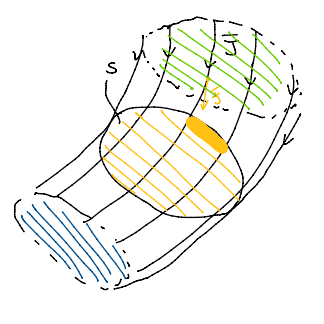
\includegraphics[scale=0.7]{immagini/image7.png}
    \end{center}

    Risulta un fascio di linee di forza. Il volume occupato dal fascio si chiama \textbf{tubo di flusso}
    \item consideriamo solo un pezzo del tubo di flusso. è caratterizzato da due superfici "tappo" ($S_A$ e $S_B$)
    \item $\nabla \overline{J} = 0 \Rightarrow \int_{\partial \tau}\overline{J}\cdot\hat{n}ds = 0$ con $\tau$ normale che esce dal volume\\
    \[\int_{S_A}\overline{J_A}\cdot\hat{n_A}ds + \int_{S_B}\overline{J_B}\cdot\hat{n_B}ds + \cancel{\int_{S_l}\overline{J_l}\cdot\hat{n_l}ds} = 0\]
    L'ultimo termine vale zero in quanto ortogonali i termini all'interno dell'integrale.\\
    Definendo $\hat{n_{B'}} = -\hat{n_B}$ e sostituendo
    \[
        \int_{S_A} \overline{J_A} \cdot \hat{n}_A \, ds - \int_{S_B} \overline{J_B} \cdot \hat{n}_{B'} \, ds = 0 \Rightarrow i_A[t, S_A] = i_B[t,S_B]
    \]
    \end{itemize}
